\chapter{Solving Strategies}
\label{chap:strategies}

This chapter describes and compares different strategies and approaches used and tested during solver development.


%%%%%%%%%%%%%%%%%%%%%%%%%%%%%%%%%%%%%%%%%%%%%%%%%%%%%%%%%%%%%%%%%%%%%%%%%%%%%%%%%%
\section{Goal programming}

Just as in any other kind of problem, the feasibility of a linear model for a timetabling problem depends utterly on data set. In general, there is no guarantee that all demanded requirements can be satisfied with the specified available resources, even because usually there are several and conflicting objectives. Therefore, specially in a commercial solver, it is important to treat some idealistic hard constraints as highest priority soft constraints, otherwise the solver could frequently generate an infeasible model.

In real life it is useless for an educational institution to have a solution that satisfies all demands of students for courses, but which does not respect some important quality requirements. Bearing this in mind, in addition to the feasibility issue, the model presented at this work, unlike most authors, does not consider demand satisfaction as a hard constraint. Essential quality requirements are modeled as hard constraints though, and demand satisfaction is treated as the highest priority objective, followed by some further goals.

While it is not easy to embody quality into the modeling process, it can be even more difficult to quantify it. A \textbf{multi-objective function} unifies disparate goals of the model in a single weighted sum of preferences. Such approach, although simpler, depends on very subjective choice of weights and is not always consistently reliable, specially when objectives are mutually conflicting.

An alternative approach is using a priority line for the different goals. According to the institution preferences, one optimizes the problem in a sequence of steps, where each step is responsible for a goal, from the most to the least important. For each step a different and specific objective function is used and the feasible solution space is subject to features of the best solution found at the previous step. Such approach is known as \textbf{preemptive goal programming} and is following detailed.


%%%%%%%%%%%%%%%%%%%%%%%%%%%%%%%%%%%%%
\subsection{General concept}

A goal programming model seeks to simultaneously take into account several objectives or goals that are concern to a decision maker. While a linear programming model consists of constraints and a single objective function to be maximized or minimized, a goal programming model consists of constraints and a set of goals that are prioritized in some sense.
In both linear and goal programming problems, if the constraints are inconsistent, there are no feasible solutions for the model. In goal programming, however, one can expect that although there is a set of feasible solutions satisfying the constraints, none of them may simultaneously satisfy all the conflicting goals of the organization. The objective of goal programming is to find a solution that satisfies the true constraints and comes closest to meeting the stated goals.

In \textbf{lexicographic} or \textbf{preemptive goal programming} the decision maker orders the unwanted deviations into a number of priority levels, with the minimization of a deviation in a higher priority level being infinitely more important than any deviations in lower priority levels. A lexicographic goal program can be solved as a series of linear programs and should be used when there is a clear priority ordering amongst the goals to be achieved. The idea behind the preemptive goal programming approach is that lower priority level goals should not be attained at the expense of higher priority goals --- they are preempted.

If the decision maker is more interested in direct comparisons of the objectives then weighted or \textbf{nonpreemptive goal programming} should be used. In this case all the unwanted deviations are multiplied by weights, reflecting their relative importance, and added together as a single sum to form the achievement function, which converts the goal programming model into a linear programming model.

G\"{u}enalay and Sahin use goal programming at \cite{Guenalay2006} to satisfy instructors' preferences as much as possible.


%%%%%%%%%%%%%%%%%%%%%%%%%%%%%%%%%%%%%
\subsection{Applying Goal Programming}

%%%%%%%%%%%%%%
\subsubsection{Preemptive Goal Programming}

Following are listed the goals, ordered by priority, considered at this work when using preemptive goal programming. For each step there is a specific objective function and the respective feasible solution space is additionally constrained by the solution of the previous phase. We draw attention to the ease of changing priorities order and adding or removing goals; and to the nonexistence of coefficients multiplying variables at each objective function.

\begin{enumerate}

%%%%%
\item{Maximizing demand satisfaction}

\begin{align*}
   \mbox{g1 = MIN  } \sum\limits_{a \in A}\sum\limits_{d \in D} fd_{d,a}
\end{align*}

%%%%%
\item{Minimizing virtual professor usage}

\begin{align*}
  \mbox{g2 = MIN  } \sum\limits_{i \in I_{d}} \sum\limits_{d \in D} \sum\limits_{cp \in CP} y_{pv,i,d,cp}
	\\
	\sum\limits_{a \in A}\sum\limits_{d \in D} fd_{d,a} \le g1
\end{align*}

Where the additional constraint restricts the solution space to the maximum demand achieved at previous step.

%%%%%
\item{Minimizing real professor displacement}

\begin{align*}
  \mbox{g3 = MIN  } \sum\limits_{p \in P} \sum\limits_{t \in T} \sum\limits_{u1 \in U} \sum\limits_{u2 \in U} Time_{u1,u2} \cdot desloc_{p,t,u1,u2}
	\\
	\sum\limits_{a \in A}\sum\limits_{d \in D} fd_{d,a} \le g1
	\\
	\sum\limits_{i \in I_{d}} \sum\limits_{d \in D} \sum\limits_{cp \in CP} y_{pv,i,d,cp} \le g2
\end{align*}

Where the additional constraint restricts the solution space to the minimum virtual professor usage achieved at previous step.

%%%%%
\item{Minimizing gaps in professor's timetable}

\begin{align*}
   \mbox{g4 = MIN  } \sum\limits_{p \in P} \sum\limits_{t \in T} \sum\limits_{f \in F} fpgap_{p,t,f}
	\\
	\sum\limits_{a \in A}\sum\limits_{d \in D} fd_{d,a} \le g1
	\\
	\sum\limits_{i \in I_{d}} \sum\limits_{d \in D} \sum\limits_{cp \in CP} y_{pv,i,d,cp} \le g2
	\\
	\sum\limits_{p \in P} \sum\limits_{t \in T} \sum\limits_{u1 \in U} \sum\limits_{u2 \in U} Time_{u1,u2} \cdot desloc_{p,t,u1,u2} \le g3
\end{align*}

Where the additional constraint restricts the solution space to the minimum real professor displacement achieved at previous step.

%%%%%
\item{Minimizing usage of further slack variables}

\begin{align*}
   \mbox{g5 = MIN  } \sum\limits_{d \in D} \sum\limits_{t \in T} \sum\limits_{i \in I_{d}} (fkp_{d,i,k} + fkm_{d,i,k})
	\\
	\sum\limits_{a \in A}\sum\limits_{d \in D} fd_{d,a} \le g1
	\\
	\sum\limits_{i \in I_{d}} \sum\limits_{d \in D} \sum\limits_{cp \in CP} y_{pv,i,d,cp} \le g2
	\\
	\sum\limits_{p \in P} \sum\limits_{t \in T} \sum\limits_{u1 \in U} \sum\limits_{u2 \in U} Time_{u1,u2} \cdot desloc_{p,t,u1,u2} \le g3
	\\
	\sum\limits_{p \in P} \sum\limits_{t \in T} \sum\limits_{f \in F} fpgap_{p,t,f} \le g4
\end{align*}


Where the additional constraint restricts the solution space to the minimum amount of gaps in professors' timetable achieved at previous step.

\end{enumerate}

The final solution is the one with cost equal to $g5$, achieved at last stage. If an optimal solution is achieved for all steps, then at the end of the last step we guarantee that the final solution found is the best one with respect to the order of priorities.


\begin{figure}[h]
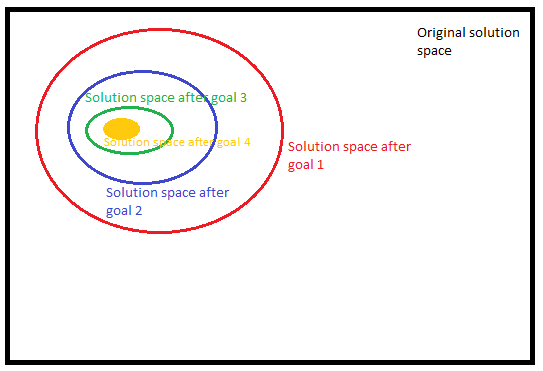
\includegraphics[scale=0.6]{figures/goalProgSpace.png}
\centering
\caption{Solution spaces are limited and encapsulated after each goal optimization step.}
\end{figure}

\fixme{atualizar etapas na figura}


%%%%%%%%%%%%%%
\subsubsection{Nonpreemptive Goal Programming}
\fixme{or Multi-objective function? no final nao tem mta diferenca!}

Following there is the unified objective function considered at this work. Although here it is even easier than at goal programming to change priorities order and adding or removing goals, there is the necessity of choosing coefficients for variables at objective function.

$$
\begin{array}{rl}
   \mbox{MIN} &
			\lambda \cdot \sum\limits_{a \in A}\sum\limits_{d \in D} \cdot fd_{d,a}
      \\
      &
      + \omega \cdot \sum\limits_{d \in D} 
\sum\limits_{t \in T} \sum\limits_{i \in I_{d}} (fkp_{d,i,k} + fkm_{d,i,k})
      \\
      &
      + \epsilon \cdot \sum\limits_{p \in P} \sum\limits_{t \in T} \sum\limits_{f \in F} fpgap_{p,t,f}
      \\
      &
			+ \sigma \cdot \sum\limits_{p \in P} \sum\limits_{t \in T} \sum\limits_{u1 \in U} \sum\limits_{u2 \in U} Time_{u1,u2} \cdot desloc_{p,t,u1,u2}
			\\
			&
      + \theta \cdot \sum\limits_{i \in I_{d}} \sum\limits_{d \in D} \sum\limits_{cp \in CP} y_{pv,i,d,cp}
\end{array}
$$


An unified objective function is more appropriate when goals have not a strict priority order, in the sense that their combinations can produce solutions that are Pareto efficient.

So, the question when choosing the approach is whether one wants to order or weight goals.


%%%%%%%%%%%%%%%%%%%%%%%%%%%%%%%%%%%%%
\subsection{Comparing results}

Through preemptive goal programming it is easier to understand the best solution found by the optimization process and the reasons of non-satisfaction of different goals, specially when the number of goals to be achieved through the objective function increases.





%%%%%%%%%%%%%%%%%%%%%%%%%%%%%%%%%%%%%%%%%%%%%%%%%%%%%%%%%%%%%%%%%%%%%%%%%%%%%%%%%%%%%%%%%%%%%%%%%%%
%%%%%%%%%%%%%%%%%%%%%%%%%%%%%%%%%%%%%%%%%%%%%%%%%%%%%%%%%%%%%%%%%%%%%%%%%%%%%%%%%%%%%%%%%%%%%%%%%%%
\section{Polishing Method}

For real-world school timetabling, where problem size is not small, solving the hole MIP introduced at section ~\ref{sec:mathForm} of chapter ~\ref{chap:mipformulation} at once with a MIP Solver like Gurobi or Cplex has been shown to be ineffective and unworkable. Tests made with an ordinary size school \fixme{falar o tamanho da escola testada} have shown that generic MIP Solvers find it already very difficult to converge to a good integer solution. For bigger schools, both the linear relaxation and the branch and bound phase are \textit{very} hard and have proven themselves impossible to be solved by current MIP solvers.

An auxiliary method was then developed for helping convergence while solving the MIP. It is described at next sections and referred here as a \q{polishing method}.


%%%%%%%%%%%%%%%%%%%%%%%%%%%%%%%
\subsection{The general idea}

Given a $lp$ model and an initial feasible solution $s$, the idea of a polishing method is iteratively to solve models $lp'$ similar but easier than the original model, such that any feasible solution for $lp'$ is also a feasible solution for $lp$ and the solution at the end of each iteration is always at least as good as at the beginning. In another words, it is generated a sequence of feasible solutions with monotonically (but not strictly) increasing quality.

Suppose that a solution $s \in \mathbb{Z}^n$ is feasible to $lp$. Let us split the set of $n$ integer variables into 2 subsets, such that $n=p+q, p \ge 0, q\ge 0$, $s_p \in \mathbb{Z}^p$, $s_q \in \mathbb{Z}^q$ and thus $s = s_p \cup s_q$. The basic principle is that optimizing a linear program $lp' = lp \cap s_p$ generates a feasible solution $s'$ to $lp'$ which is also feasible to $lp$ and at least as good as $s$. All variables and constraints of the original problem are still present in the new problem, but cuts were added, which limit the solution space based on $s_p$, resulting in a more restricted solution space. The smaller is the solution space, the easier is the solver convergence.

The aim of cutting the solution space here is not to eliminate non-promising search-space regions, but to search in a smaller and treatable space. There is then no guarantee that the actual optimal solution $s*$ for $lp$ is in or out the eliminated region, but it is ensured that the optimal solution $s'*$ for $lp'$ is equal or better than the previously known solution $s$. It is thus not interesting to keep these cuts after solving $lp'$. Instead, the idea is to restore the original problem and add others cuts, now based on the new solution $s'$. Doing that iteratively, we create a guide for the solver.

So, what solution space of $lp'$ looks like? At each polishing iteration, the limitation of the search-space takes place through the tightening of a subset of variables bounds based on the initial solution $s$. Suppose the trivial example where the solution space is equal to the cube $c = [0, 4]^3 \in \mathbb{Z}^3$ and the feasible solution $s \in \mathbb{Z}^3$ is $s = \{s_1=3,s_2=2,s_3=0\}$. A possible limitation based on $s$ would be to tighten the interval bounds of the first dimension to the value of $s_1$, such that the resulting solution space is $c' = [3, 3][0, 4][0, 4]$. Such tightening clearly eliminates one dimension of the search-space and keeps the feasible solution $s$. Consequently, optimizing over $c'$ can not lead to a worse solution, because in the worst-case scenario the best solution is $s$ itself.

Because at the beginning of the polishing process the solution is supposedly a very poor quality one and the search-space is a wide unexplored space, the percentage of variables with tightened bounds starts high (lets say around 90\%) and drops as the limited search-space is potentially exhausted and solution improvement stagnates. If at the end of the polishing this percentage reaches 0\%, then the considered linear program is the original one and its optimization ends the process. If an optimal solution is found at the 0\% stage, then it is surely an optimal solution for the original problem. For too hard linear programs though, it is unlikely that the polishing reaches this last stage, and the process is then interrupted by time limit. Generally speaking, nothing can be said about optimality for a solution found before the 0\% stage.



%%%%%%%%%%%%%%%%%%%%%%%%%%%%%%%%%%%%%
\subsection{The polishing algorithm developed for the problem}

Following a detailed pseudo-algorithm for the polishing method developed for the school timetabling problem is described. The main algorithm, specified at ~\ref{alg:polishing}, contains the general steps of the polishing process.

The essential requirements for using the polishing method are a linear program and a feasible initial solution. In addition, run time limits are used as stopping criteria: a total maximum execution time for the method ($maxTime$); and a maximum execution time since the last solution improvement occurrence ($maxTimeNoImprov$).

The algorithm starts at line ~\ref{polish:ln:init} with some initialization, defined at ~\ref{alg:init}. The current solution $sol$ is set with the initial solution, the percentage $perc$ of variables with fixed bounds is initialized with 90\%, the MIP optimization time limit $timeIter$ is initialized with 70 seconds and, in the case of several blocks which share teaching resources, blocks may be clustered to assist further bounds tightening. The polishing process begins at line ~\ref{polish:ln:iter}, where at each iteration a new optimization cycle takes place. Every cycle has 4 main steps: variables bounds tightening (line ~\ref{polish:ln:fix}), optimization of the tightened linear program (line ~\ref{polish:ln:opt}), update of percentage of fixed variables and of time limit for each optimization (line ~\ref{polish:ln:perc}), and variables bounds release (line ~\ref{polish:ln:unfix}). At line ~\ref{polish:ln:runtime} the polishing run time limit is checked.


\begin{algorithm}[H]
  \caption{Polishing method
    \label{alg:polishing}} 
  \begin{algorithmic}[1]
    \Require{$lp$ model, any initial feasible solution $solIni$, the maximum run time $maxTime$ for the hole polishing method and the maximum run time $maxTimeNoImprov$ of polishing without improvement}
		\Ensure{A final feasible solution $sol$ for the $lp$ model at least as good as the initial solution $solIni$}
    \Statex
    \Function{Polish}{$solIni$, $maxTime$, $maxTimeNoImprov$}		
			\State \textsc{init}$()$																	\label{polish:ln:init}
			\Let{$okIter$}{$true$}
      \While{$okIter$}																					\label{polish:ln:iter}
          \State \textsc{fixVars}$()$														\label{polish:ln:fix}
					\State \textsc{optimize}$()$													\label{polish:ln:opt}
					\State \textsc{updatePercAndTimeIter}$()$							\label{polish:ln:perc}
					\State \textsc{unfixVars}$()$													\label{polish:ln:unfix}
					\State \textsc{checkRunTimeLimit}$()$									\label{polish:ln:runtime}
      \EndWhile
     \State \Return{$sol$}
    \EndFunction
	\Statex	
  \Algphase{Initialization}
    \Procedure{init}{$lp$, $solIni$}														\label{alg:init}
				\Let{$sol$}{$solIni$}
				\Let{$perc$}{$90$}
				\Let{$timeIter$}{70}
				\State cluster blocks according to teaching staff sharing
    \EndProcedure
  \end{algorithmic}
\end{algorithm}		
		
		
		
		
\begin{algorithm}[H]
  \caption{Fixing variables' values
    \label{alg:fixVars}}
  \begin{algorithmic}[1]
    \Require{$lp$ model, a feasible solution $sol$ and the percentage $perc$ of classes variables to fix}
		\Ensure{A resultant lp model with a random subset of its variables with fixed bounds and therefore easier to solve}
    \Procedure{fixVars}{}
			\State \textsc{fixBlocks}$()$
			\Let {$F$}{\textsc{decideVarsToFix}$()$}
			\State \textsc{fixVarsBounds}$()$
			\State \textsc{fixVarsProfBounds}$()$
    \EndProcedure
	\Statex	
  \Algphase{Fixing blocks}
    \Require{$lp$ model, a feasible solution $sol$ and a set $FB$ of fixed blocks}
    \Procedure{fixBlocks}{}
			 \For{each variable $x_{u} \in lp$ such that $u \in FB$}
				\Let{$lowerbound_{x}$}{$sol[x]$}
				\Let{$upperbound_{x}$}{$sol[x]$} 
			 \EndFor
    \EndProcedure
	\Statex
  \Algphase{Decide which variable to fix}
    \Require{$lp$ model, a feasible solution $sol$ and a percentage $perc$ of classes to be fixed}
		\Ensure{Returns a subset $F$ of classes to be fixed}
    \Function{decideVarsToFix}{}
			\Let{$F$}{$\emptyset$}
			\For{each variable $z \in lp$}
					\If{$rand() \ge perc$}
						\Let{$F$}{class represented by $z$}
					\EndIf
			\EndFor
			\Return F
    \EndFunction
	\Statex
	\Algphase{Fix bounds of variables of lessons}
    \Require{$lp$ model, a feasible solution $sol$ and a set $F$ of classes to be fixed}
    \Procedure{fixVarsBounds}{}
			 \For{each variable $x \in lp$ such that class of $x$ is in $F$}
				\Let{$lowerbound_{x}$}{$sol[x]$}
				\Let{$upperbound_{x}$}{$sol[x]$} 
			 \EndFor
    \EndProcedure	
	\Statex
	\Algphase{Fix bounds of variables of professors}
    \Require{$lp$ model and a feasible solution $sol$}
    \Procedure{fixVarsProfBounds}{}
			\For{each variable $y \in lp$}
					\If{$rand() \ge perc$}
						\Let{$lowerbound_{y}$}{$sol[y]$}
						\Let{$lowerbound_{y}$}{$sol[y]$} 
					\EndIf
			\EndFor
    \EndProcedure	
  \end{algorithmic}	
\end{algorithm}


\begin{algorithm}[H]
  \caption{Optimize
    \label{alg:optimize}}
  \begin{algorithmic}[1]
    \Require{$lp$ model, a feasible solution $sol$ to $lp$}
		\Ensure{A final updated feasible solution $sol$ for the $lp$ model at least as good as the initial solution}
    \Procedure{optimize}{}
			\State set optimization time limit equal to $timeIter$
			\State set $sol$ as a start solution to $lp$	
			\State optimize $lp$
			\Let{$runtime$}{run time spent at the optimization}
			\Let{$timeLeft$}{\abs{timeIter - runtime}}
			\If{optimization succeeded}
				\Let{$sol$}{new best solution found}
			\EndIf
    \EndProcedure	
  \end{algorithmic}	
\end{algorithm}		


\begin{algorithm}[H]
  \caption{Update percentage of fixed variables, fixed blocks and maximum time per iteration
    \label{alg:updatePercAndTimeIter}}
  \begin{algorithmic}[1]
    \Require{$lp$ model}
    \Procedure{updatePercAndTimeIter}{}
			\If{\textsc{allFree}$()$}
				\Let{$okIter$}{$false$}
				\Return
			\EndIf
			\State \textsc{updateIterSemMelhora}$()$
	    \If {\textit{lp was solved until optimal or gap is small enough}}
			  \State \textsc{updatePercAndTimeIterSmallGap}$()$
			\Else
				\State \textsc{updatePercAndTimeIterBigGap}$()$
			\EndIf
	    \If{\textsc{allFree}$()$}
				\Let{$timeIter$}{\textsc{getLeftTime$()$}}
			\EndIf
    \EndProcedure	
		\Statex
		\Algphase{Update percentage of fixed variables, fixed blocks and maximum time per iteration for small gap case}
			\Procedure{updatePercAndTimeIterSmallGap}{}
				\If{\textsc{allFree}$()$}
				\Let{okIter}{false}
				\EndIf
				\State \textsc{adjustPercOrBlock}()
				\State \textsc{adjustTime}()
			\EndProcedure
		\Statex
		\Algphase{Update percentage of fixed variables, fixed blocks and maximum time per iteration for big gap case}
			\Procedure{updatePercAndTimeIterBigGap}{}
				\If{solution was not improved at the current iteration}
					\Let{$acresm$}{0, if all blocks are currently free; or 10 otherwise}
					\State \textsc{setNextRandFreeBlocks}$(acresm)$
					\State \textsc{adjustTime}()
				\EndIf
			\EndProcedure			
  \end{algorithmic}	
\end{algorithm}


\begin{algorithm}[H]
  \caption{Set free and fixed blocks for the next iteration
    \label{alg:setNextRandFreeBlocks}}
  \begin{algorithmic}[1]
    \Require{$lp$ model}
    \Statex
    \Procedure{setNextRandFreeBlocks}{$percAdjust$}
			\Let{$percBlockFixed$}{$percBlockFixed + percAdjust$} 	%\Comment{update percentage of fixed blocks for next iteration}
      \If{there is enough consecutive iterations with fixed blocks}
      	\State free all blocks for the next iteration
      	\Return
      \EndIf
      \State \textsc{chooseAndSetFreeBlocks}()
    \EndProcedure
	  \Statex
	  \Algphase{Choose and set free blocks for the next iteration}
    \Procedure{chooseAndSetFreeBlocks}{}
			\State reset free blocks
			\Let{useCluster}{true or false, randomly chosen with $50\%$ of chance of true}
			\If{useCluster} 																					%\Comment{type of fixing blocks is per cluster}
				\State choose a cluster of blocks and set it free
			\EndIf
			\While{number of free blocks $<$ $(100-percBlockFixed)\cdot$ \textit{total of blocks}}
			\State choose randomly a block and set it free
			\EndWhile
    \EndProcedure
  \end{algorithmic}
\end{algorithm}


\begin{algorithm}[H]
  \caption{Adjust time
    \label{alg:adjustTime}}
  \begin{algorithmic}[1]
    \Require{$lp$ model}
    \Procedure{adjustTime}{}
			\If {solution was not improved at the current iteration \textbf{and} time limit for the iteration was reached}
				\State \textsc{increaseTime}()													%\Comment{time limit reached  increases time limit}
			\EndIf
			\If {solution was improved at the current iteration}
				\State \textsc{decreaseTime}()													%\Comment{Adjust time limit in case it is too high}
			\EndIf
    \EndProcedure	
	  \Statex
	  \Algphase{Increase time}
    \Procedure{increaseTime}{}
			\Let{$incremTime$}{10}																		%	\Comment{increases the time limit by a fixed amount}
			\Let{$incremTime$}{$incremTime + (100-perc)\cdot 0.2$}		%\Comment{increases the time limit the more perc is close to 0}
			\Let{$incremTime$}{$incremTime + (100-percBlockFixed)\cdot 0.2$}	%\Comment{increases the time limit the more blocks are free}
			\Let{$timeIter$}{$timeIter + incremTime$}
			\If{$timeIter > MaxTimeImposedPerIteration$}
				\Let{$timeIter$}{$MaxTimeImposedPerIteration$} 					%\Comment{possibly forces a reduction of $timeIter$, whether a maximum time per iteration is imposed.}
			\EndIf
    \EndProcedure	
	  \Statex
	  \Algphase{Decrease time}
    \Procedure{decreaseTime}{}
			\If{\textsc{allFree}$()$}
				\Let{$timeIter$}{$getLeftTime()$}												%\Comment{next iteration will be the last one}
			\Else
				\Let{$minExcess$}{$max(0.5\cdot timeIter, 50)$}
				\If{$timeLeft > minExcess$} 														%\Comment{Adjust time limit in case it is too high}
					\Let{$timeIter$}{$runtime+minExcess$}
				\EndIf
			\EndIf
    \EndProcedure			
  \end{algorithmic}
\end{algorithm}


\begin{algorithm}[H]
  \caption{Adjust percentage of fixed variables or fixed blocks
    \label{alg:adjustPercOrBlock}}
  \begin{algorithmic}[1]
    \Require{$lp$ model}
    \Procedure{adjustPercOrBlock}{}
			\If{$optimal$ \textbf{and} $timeLeft > 0.7\cdot timeIter$}	%\Comment{decrease the fixed portion if it was easy (fast) to solve}
				\State \textsc{decreasePercOrFreeBlock}$(5)$	
			\Else 
				\If{\textbf{not} $improved$}																%\Comment{decrease the fixed portion if no improvement was made}	
					\State \textsc{decreasePercOrFreeBlock}$(10)$		
				\EndIf	
			\EndIf
    \EndProcedure	
	  \Statex
	  \Algphase{Decrease percentage of fixed variables or free blocks}
    \Procedure{decreasePercOrFreeBlock}{$percToSubtract$}
			\If{$percToSubtract \le 0$}
				\Return
			\EndIf
			\If{there is any block currently fixed}
				\State \textsc{setNextRandFreeBlock}$(-10)$
				\Return
			\EndIf
			\State \textsc{decreasePerc}$(percToSubtract)$
    \EndProcedure
  \end{algorithmic}
\end{algorithm}


\begin{algorithm}[H]
  \caption{Unfixing variables' values
    \label{alg:unfixVars}}
  \begin{algorithmic}[1]
    \Require{$lp$ model}
    \Procedure{unfixVars}{}
			\For{each variable $var\in lp$ that was fixed}
					\Let{$lowerbound_{var}$}{\textit{original lower bound of var}}
					\Let{$upperbound_{var}$}{\textit{original upper bound of var}}
			\EndFor
    \EndProcedure	
  \end{algorithmic}	
\end{algorithm}


\begin{algorithm}[H]
  \caption{Check run time
    \label{alg:checktime}}
  \begin{algorithmic}[1]
    \Require{$lp$ model}
    \Procedure{checkRunTimeLimit}{}
			\State \textsc{checkTotalRunTime}()
			\State \textsc{checkTimeWithoutImprov}()
    \EndProcedure		
		\Statex
	  \Algphase{Check total run time}
    \Procedure{checkTotalRunTime}{}
			\If{total run time $\ge$ maxTime} % maximum run time allowed for polishing
					\Let{$okIter$}{$false$}
			\EndIf
    \EndProcedure	
		\Statex
	  \Algphase{Check run time since last improvement}
    \Procedure{checkTimeWithoutImprov}{}
			\If{no improvement was made at the current iteration}
				\If{run time since last improvement $>$ maxTimeNoImprov} % maximum run time allowed without improvement
					\Let{$okIter$}{$false$}
				\EndIf
			\Else
				\State reset time without improvement 
			\EndIf		
		\EndProcedure	
  \end{algorithmic}	
\end{algorithm}





%%%%%%%%%%%%%%%%%%%%%%%%%%%%%%%%%%%%%

\subsection{Comparing different approaches}

%%%%%%%%%%%%%%%%%%%%%%%%%%%%%%%%%%%%%
\subsubsection{Fixing types}




%%%%%%%%%%%%%%%%%%%%%%%%%%%%%%%%%%%%%%%%%%%%%%%%%%%%%%%%%%%%%%%%%%%%%%%%%%%%%%%%%%%%%%%%%%%%%%%%%%%
%%%%%%%%%%%%%%%%%%%%%%%%%%%%%%%%%%%%%%%%%%%%%%%%%%%%%%%%%%%%%%%%%%%%%%%%%%%%%%%%%%%%%%%%%%%%%%%%%%%
\section{Root relaxation}

%%%%%%%%%%%%%%%%%%%%%%%%%%%%%%%%%%%%%
\subsection{Barrier method vs primal method algorithms}




%%%%%%%%%%%%%%%%%%%%%%%%%%%%%%%%%%%%%%%%%%%%%%%%%%%%%%%%%%%%%%%%%%%%%%%%%%%%%%%%%%%%%%%%%%%%%%%%%%%
%%%%%%%%%%%%%%%%%%%%%%%%%%%%%%%%%%%%%%%%%%%%%%%%%%%%%%%%%%%%%%%%%%%%%%%%%%%%%%%%%%%%%%%%%%%%%%%%%%%
\section{Different mathematical formulation}

%%%%%%%%%%%%%%%%%%%%%%%%%%%%%%%%%%%%%
\subsection{Single time slot variable vs grouping time slot variable}



As in all combinatorial scheduling models, the problem grows more complex as the number of side constraints increases.\fixme{Colocar essa frase no lugar adequado!}



%%%%%%%%%%%%%%%%%%%%%%%%%%%%%%%%%%%%%%%%%%%%%%%%%%%%%%%%%%%%%%%%%%%%%%%%%%%%%%%%%%%%%%%%%%%%%%%%%%%
%%%%%%%%%%%%%%%%%%%%%%%%%%%%%%%%%%%%%%%%%%%%%%%%%%%%%%%%%%%%%%%%%%%%%%%%%%%%%%%%%%%%%%%%%%%%%%%%%%%
\section{Usage of virtual resource}

%%%%%%%%%%%%%%%%%%%%%%%%%%%%%%%%%%%%%
\subsection{Virtual professor vs no virtual professors}

